%Version 3 December 2023
% See section 11 of the User Manual for version history
%
%%%%%%%%%%%%%%%%%%%%%%%%%%%%%%%%%%%%%%%%%%%%%%%%%%%%%%%%%%%%%%%%%%%%%%
%%                                                                 %%
%% Please do not use \input{...} to include other tex files.       %%
%% Submit your LaTeX manuscript as one .tex document.              %%
%%                                                                 %%
%% All additional figures and files should be attached             %%
%% separately and not embedded in the \TeX\ document itself.       %%
%%                                                                 %%
%%%%%%%%%%%%%%%%%%%%%%%%%%%%%%%%%%%%%%%%%%%%%%%%%%%%%%%%%%%%%%%%%%%%%

%%\documentclass[referee,sn-basic]{sn-jnl}% referee option is meant for double line spacing

%%=======================================================%%
%% to print line numbers in the margin use lineno option %%
%%=======================================================%%

%\documentclass[lineno,sn-basic]{sn-jnl}% Basic Springer Nature Reference Style/Chemistry Reference Style

%%======================================================%%
%% to compile with pdflatex/xelatex use pdflatex option %%
%%======================================================%%

%%\documentclass[pdflatex,sn-basic]{sn-jnl}% Basic Springer Nature Reference Style/Chemistry Reference Style


%%Note: the following reference styles support Namedate and Numbered referencing. By default the style follows the most common style. To switch between the options you can add or remove “Numbered in the optional parenthesis. 
%%The option is available for: sn-basic.bst, sn-vancouver.bst, sn-chicago.bst%  
 
%%\documentclass[pdflatex,sn-nature]{sn-jnl}% Style for submissions to Nature Portfolio journals
%%\documentclass[pdflatex,sn-basic]{sn-jnl}% Basic Springer Nature Reference Style/Chemistry Reference Style
%\documentclass[lineno,pdflatex,sn-mathphys-num]{sn-jnl}% Math and Physical Sciences Numbered Reference Style 

\documentclass[drones,technicalnote,accept,pdftex,moreauthors]{Definitions/mdpi} 
\linenumbers

%%\documentclass[pdflatex,sn-mathphys-ay]{sn-jnl}% Math and Physical Sciences Author Year Reference Style
%%\documentclass[pdflatex,sn-aps]{sn-jnl}% American Physical Society (APS) Reference Style
%%\documentclass[pdflatex,sn-vancouver,Numbered]{sn-jnl}% Vancouver Reference Style
%%\documentclass[pdflatex,sn-apa]{sn-jnl}% APA Reference Style 
%%\documentclass[pdflatex,sn-chicago]{sn-jnl}% Chicago-based Humanities Reference Style

%%%% Standard Packages 
%%<additional latex packages if required can be included here>

\usepackage{graphicx}%
\usepackage{multirow}%
\usepackage{amsmath,amssymb,amsfonts}%
\usepackage{amsthm}%
\usepackage{mathrsfs}%
\usepackage[title]{appendix}%
\usepackage{xcolor}%
\usepackage{textcomp}%
\usepackage{manyfoot}%
\usepackage{booktabs}%
\usepackage{algorithm}%
\usepackage{algorithmicx}%
\usepackage{algpseudocode}%
\usepackage{listings}%
%%%%

%%%%%=============================================================================%%%%
%%%%  Remarks: This template is provided to aid authors with the preparation
%%%%  of original research articles intended for submission to journals published 
%%%%  by Springer Nature. The guidance has been prepared in partnership with 
%%%%  production teams to conform to Springer Nature technical requirements. 
%%%%  Editorial and presentation requirements differ among journal portfolios and 
%%%%  research disciplines. You may find sections in this template are irrelevant 
%%%%  to your work and are empowered to omit any such section if allowed by the 
%%%%  journal you intend to submit to. The submission guidelines and policies 
%%%%  of the journal take precedence. A detailed User Manual is available in the 
%%%%  template package for technical guidance.
%%%%%=============================================================================%%%%

%\newcommand{\absdiv}[1]{%
%  \par\addvspace{.5\baselineskip}% adjust to suit
%  \noindent\textbf{#1}\quad\ignorespaces
%}

%% as per the requirement new theorem styles can be included as shown below
%\theoremstyle{thmstyleone}%
%\newtheorem{Theorem}{Theorem}%  meant for continuous numbers
%%%\newtheorem{Theorem}{Theorem}[section]% meant for sectionwise numbers
%%% optional argument [theorem] produces theorem numbering sequence instead of independent numbers for Proposition
%\newtheorem{Proposition}[theorem]{Proposition}% 
%%%\newtheorem{Proposition}{Proposition}% to get separate numbers for theorem and proposition etc.
%
%\theoremstyle{thmstyletwo}%
%\newtheorem{Example}{Example}%
%\newtheorem{Remark}{Remark}%
%
%\theoremstyle{thmstylethree}%
%\newtheorem{Definition}{Definition}%
%
%\raggedbottom
%%\unnumbered% uncomment this for unnumbered level heads

%=================================================================
% MDPI internal commands - do not modify
\firstpage{1} 
\makeatletter 
\setcounter{page}{\@firstpage} 
\makeatother
\pubvolume{1}
\issuenum{1}
\articlenumber{0}
\pubyear{2026}
\copyrightyear{2025}
%\externaleditor{Firstname Lastname} % More than 1 editor, please add `` and '' before the last editor name
\datereceived{ } 
\daterevised{ } % Comment out if no revised date
\dateaccepted{ } 
\datepublished{ } 
%\datecorrected{} % For corrected papers: "Corrected: XXX" date in the original paper.
%\dateretracted{} % For retracted papers: "Retracted: XXX" date in the original paper.
%\hreflink{https://doi.org/} % If needed use \linebreak
%\doinum{}
%\pdfoutput=1 % Uncommented for upload to arXiv.org
%\CorrStatement{yes}  % For updates
%\longauthorlist{yes} % For many authors that exceed the left citation part
%\IsAssociation{yes} % For association journals

%=================================================================
% Full title of the paper (Capitalized)
\Title{\textsc{drone2report}: A Configuration-Driven Multi-Sensor Pipeline for UAV-Based Crop Phenotyping and Precision Agriculture}



%\title[Article Title]{\textsc{drone2report}: a configuration-driven multi-sensor pipeline for UAV-based crop phenotyping and precision agriculture}

%%=============================================================%%
%% GivenName	-> \fnm{Joergen W.}
%% Particle	-> \spfx{van der} -> surname prefix
%% FamilyName	-> \sur{Ploeg}
%% Suffix	-> \sfx{IV}
%% \author*[1,2]{\fnm{Joergen W.} \spfx{van der} \sur{Ploeg} 
%%  \sfx{IV}}\email{iauthor@gmail.com}
%%=============================================================%%

% Author Orchid ID: enter ID or remove command
\newcommand{\orcidauthorA}{0000-0003-2710-9885} % Add \orcidA{} behind the author's name
%\newcommand{\orcidauthorB}{0000-0000-0000-000X} % Add \orcidB{} behind the author's name

% Authors, for the paper (add full first names)
\Author{Nelson Nazzicari $^{1,}$*\orcidA{}, Giulia Moscatelli $^{2}$, Agostino Fricano $^{3}$, Elisabetta Frascaroli $^{4}$, Roshan Paudel $^{4}$, Eder Groli $^{5}$, Paolo De Franceschi $^{5}$, Giorgia Carletti $^{3}$, Nicolo Franguelli $^{1}$ and Filippo Biscarini $^{2}$}

%\longauthorlist{yes}

% MDPI internal command: Authors, for metadata in PDF
\AuthorNames{Nelson Nazzicari, Giulia Moscatelli, Agostino Fricano, Elisabetta Frascaroli, Roshan Paudel, Eder Groli, Paolo De Franceschi, Giorgia Carletti, Nicolo Franguelli and Filippo Biscarini}

% Affiliations / Addresses (Add [1] after \address if there is only one affiliation.)
\address{%
$^{1}$ \quad Research Centre for Animal Production and Aquaculture, Council for Agricultural Research and Analysis of Agricultural Economics, Viale Piacenza, 29, {Lodi}, {26900}, {Italy}; nicolo.franguelli@crea.gov.it\\
$^{2}$ \quad Institute of Biology and Biotechnology in Agriculture (IBBA), National Research Council (CNR), {Via A. Corti, 12}, {Milan}, {20133}, {Italy}; giulia.moscatelli@ibba.cnr.it; filippo.biscarini@cnr.it\\
$^{3}$ \quad Research Centre for Genomics and Bioinformatics, Council for Agricultural Research and Analysis of Agricultural Economics, {Via San Protaso 69}, {Fiorenzuola d'Arda}, {29017}, {Italy}; giulia.moscatelli@ibba.cnr.it; giorgia.carletti@crea.gov.it\\
$^{4}$ \quad Department of Agricultural and Food Sciences, University of Bologna, {Via G. Fanin, 44}, {Bologna}, {40127}, {Italy}; elisabetta.frascaroli@unibo.it; roshan.paudel@unibo.it\\
$^{5}$ \quad Research \& Development, SIS - Società Italiana Sementi, {Via Mirandola, 5}, {San Lazzaro di Savena (BO)}, {40068}, {Italy}; e.groli@sisonweb.com; p.defranceschi@sisonweb.com}

% Contact information of the corresponding author
\corres{Correspondence: nelson.nazzicari@crea.gov.it}

%\author*[1]{\fnm{Nelson} \sur{Nazzicari}}\email{nelson.nazzicari@crea.gov.it}\email{https://orcid.org/0000-0003-2710-9885}
%
%\author[2]{\fnm{Giulia} \sur{Moscatelli}}\email{giulia.moscatelli@ibba.cnr.it}
%
%\author[3]{\fnm{Agostino} \sur{Fricano}}\email{agostino.fricano@crea.gov.it}
%
%\author[4]{\fnm{Elisabetta} \sur{Frascaroli}}\email{elisabetta.frascaroli@unibo.it}
%
%\author[4]{\fnm{Roshan} \sur{Paudel}}\email{roshan.paudel@unibo.it}
%
%\author[5]{\fnm{Eder} \sur{Groli}}\email{e.groli@sisonweb.com}
%
%\author[5]{\fnm{Paolo} \sur{De Franceschi}}\email{p.defranceschi@sisonweb.com }
%
%\author[3]{\fnm{Giorgia} \sur{Carletti}}\email{giorgia.carletti@crea.gov.it}
%
%\author[1]{\fnm{Nicolo} \sur{Franguelli}}\email{nicolo.franguelli@crea.gov.it}
%
%\author[2]{\fnm{Filippo} \sur{Biscarini}}\email{filippo.biscarini@cnr.it}

%\affil[1]{\orgdiv{Research Centre for Animal Production and Aquaculture}, \orgname{Council for Agricultural Research and Analysis of Agricultural Economics}, \orgaddress{\street{Viale Piacenza, 29}, \city{Lodi}, \postcode{26900}, \country{Italy}}}
%
%\affil[2]{\orgdiv{Institute of Biology and Biotechnology in Agriculture (IBBA)}, \orgname{National Research Council (CNR)}, \orgaddress{\street{Via A. Corti, 12}, \city{Milan}, \postcode{20133}, \country{Italy}}}
%
%\affil[3]{\orgdiv{Research Centre for Genomics and Bioinformatics}, \orgname{Council for Agricultural Research and Analysis of Agricultural Economics}, \orgaddress{\street{Via San Protaso 69}, \city{Fiorenzuola d'Arda}, \postcode{29017}, \country{Italy}}}
%
%\affil[4]{\orgdiv{Department of Agricultural and Food Sciences}, \orgname{University of Bologna}, \orgaddress{\street{Via G. Fanin, 44}, \city{Bologna}, \postcode{40127}, \country{Italy}}}
%
%\affil[5]{\orgdiv{Research \& Development}, \orgname{SIS - Società Italiana Sementi}, \orgaddress{\street{Via Mirandola, 5}, \city{San Lazzaro di Savena (BO)}, \postcode{40068}, \country{Italy}}}
\addhighlights{yes}
\renewcommand{\addhighlights}{%
\noindent\vspace{3pt}\\
\textbf{What are the main fundings?}
\begin{itemize}[labelsep=2.5mm,topsep=-3pt]
\item UAV imagery plays an ever-growing role in agriculture, particularly in breeding and crop monitoring.
\item Data-processing pipelines are typically a mixture of standard and custom software, leading to inconsistencies and difficulties in reproducibility.
\end{itemize}\vspace{3pt}
\textbf{What are the implications of the main findings?}
\begin{itemize}[labelsep=2.5mm,topsep=-3pt]
\item A new dedicated library, DRONE2REPORT, is released as a standardized and customizable open-source  framework for processing UAV images in agriculture.
\item We demonstrate a wide range of applicability and integration, covering both traditional approaches (e.g. vegetation indices) and innovative techniques (e.g. deep learning and computer vision).
\end{itemize}
}
%%==================================%%
%% Sample for unstructured abstract %%
%%==================================%%

\abstract{\textbf{Background}: Unmanned aerial vehicles (UAVs) have become indispensable tools in precision agriculture and plant phenotyping, enabling rapid, non-destructive assessment of crop traits across space and time. Equipped with RGB, multispectral, thermal, and other sensors, UAVs provide detailed information on canopy structure, physiology, and stress responses that can guide management decisions and accelerate breeding programs. Despite these advances, the downstream processing of UAV imagery remains technically demanding. Converting orthophotos into standardized, biologically meaningful data often requires a combination of photogrammetry, geospatial analysis, and custom scripting, which can limit reproducibility and accessibility across research groups. \textbf{Results}: We present \textsc{drone2report}, an open-source python-based software that processes orthophotos/orthomosaics from UAV flights to generate vegetation indices, summary statistics and derived subimages, supporting both research and applied breeding contexts. Alongside the basic structure and functioning of \textsc{drone2report}, we present also five case studies that illustrate practical applications common in UAV/drone-phenotyping of plants: i) thresholding to remove background noise and highlight regions of interest; ii) monitoring plant phenotypes over time; iii) extracting information on plant height to detect events like lodging; iv) integrating multiple sensors (cameras) to construct and optimise new synthetic indices; v) integrate a trained deep learning network to implement a classification task.
These examples demonstrate the tool’s ability to automate analysis, integrate heterogeneous data and models, and support reproducible computation of agronomically relevant traits. \textbf{Conclusions}: \textsc{drone2report}  streamlines UAV image processing for precision agriculture by linking orthophoto data to standardized, plot-level outputs. Its modular, configuration-driven design allows transparent workflows, easy customization, and integration of multiple sensors within a unified analytical framework. By facilitating reproducible, multi-modal image analysis, drone2report lowers technical barriers to UAV-based phenotyping and opens the way to robust, data-driven crop monitoring and breeding applications.
}

%%================================%%
%% Sample for structured abstract %%
%%================================%%

% \abstract{\textbf{Purpose:} The abstract serves both as a general introduction to the topic and as a brief, non-technical summary of the main results and their implications. The abstract must not include subheadings (unless expressly permitted in the journal's Instructions to Authors), equations or citations. As a guide the abstract should not exceed 200 words. Most journals do not set a hard limit however authors are advised to check the author instructions for the journal they are submitting to.
% 
% \textbf{Methods:} The abstract serves both as a general introduction to the topic and as a brief, non-technical summary of the main results and their implications. The abstract must not include subheadings (unless expressly permitted in the journal's Instructions to Authors), equations or citations. As a guide the abstract should not exceed 200 words. Most journals do not set a hard limit however authors are advised to check the author instructions for the journal they are submitting to.
% 
% \textbf{Results:} The abstract serves both as a general introduction to the topic and as a brief, non-technical summary of the main results and their implications. The abstract must not include subheadings (unless expressly permitted in the journal's Instructions to Authors), equations or citations. As a guide the abstract should not exceed 200 words. Most journals do not set a hard limit however authors are advised to check the author instructions for the journal they are submitting to.
% 
% \textbf{Conclusion:} The abstract serves both as a general introduction to the topic and as a brief, non-technical summary of the main results and their implications. The abstract must not include subheadings (unless expressly permitted in the journal's Instructions to Authors), equations or citations. As a guide the abstract should not exceed 200 words. Most journals do not set a hard limit however authors are advised to check the author instructions for the journal they are submitting to.}

\keyword{drone phenotyping; image processing; software package; precision agriculture; UAV; vegetation index; NDVI; deep learning; neural networks}

%%\pacs[JEL Classification]{D8, H51}

%%\pacs[MSC Classification]{35A01, 65L10, 65L12, 65L20, 65L70}

\begin{document}

%\maketitle
\section{Introduction}
\label{intro}
Advances in precision agriculture and plant phenotyping increasingly rely on high-throughput, non-destructive methods for measuring crop performance under field conditions. Remote sensing platforms have become central to this effort, providing quantitative information on canopy structure, physiology, and stress responses. Among them, unmanned aerial vehicles (UAVs, or drones) are especially attractive due to their flexibility, affordability, and ability to generate repeated observations at plot or field scale. UAV-mounted sensors—ranging from RGB cameras to multispectral, thermal, and LIDAR (Laser Imaging, Detection, And Ranging) units—enable detailed measurement of vegetation indices, canopy temperature, and topography that can inform breeding programs and management decisions \cite{machwitz2021bridging}.

Although the potential of UAV imagery for plant science is well recognized, the software ecosystem supporting its analysis remains fragmented. Many researchers rely on commercial photogrammetry suites for orthomosaic production, followed by manual processing in GIS software or custom scripts for index calculation and region-of-interest (ROI) extraction. This workflow can be labor-intensive, error-prone, and difficult to reproduce across experiments or research groups. Existing open-source solutions are usually not designed for agriculture applications (\cite{moyroud2018introduction}), have sometimes very specific targets (e.g. seeds \cite{tang2024grabseeds}, berries \cite{loarca2024berryportraits}), focus on single data types (e.g. RGB or multispectral), provide limited support for multi-modal datasets, or lack transparent configuration and automation mechanisms. 

As UAV datasets grow in size and complexity, there is a growing need for tools that combine reproducibility, flexibility, and ease of use, while remaining accessible to plant researchers without advanced programming expertise.
\textsc{drone2report} was developed to address this gap. It is designed specifically for agriculture (\textit{e.g.} a field with multiple plots each accommodating one genotype) and implements a configuration-driven pipeline that streamlines the transformation of UAV imagery into standardized outputs—such as vegetation indices, ROI-based statistics, and summary reports—across multiple sensor types. By emphasizing reproducibility, modularity, and compatibility with common research workflows, \textsc{drone2report} aims to lower the barrier to adoption of UAV-based phenotyping and facilitate robust comparisons across experiments, genotypes, and environments. 
%The software is released under open-source license and readily available at \url{https://github.com/ne1s0n/drone2report}. 
In this paper, we present the technical details of this new tool, followed by four case-studies describing examples of its application, a comparison with other available software packages, and a discussion of the merits, limitations and future expansions of \textsc{drone2report}.

\section{Methods}
\label{methods}

\subsection{Data Workflow}
The general workflow of \textsc{drone2report} is reported in Figure~\ref{fig:workflow}. 
We adopt here the following definitions: orthophotos (or orthorectified images) are single drone-captured images that have been geometrically corrected (perspective, camera tilt etc.), while orthomosaics are collection of orthophotos stitched together (taking care of overlaps etc.) \cite{park2022deep}.
The first step is data acquisition, with the drone(s) flying over the field of interest and collecting a series of overlapping images, which are then collated together into an orthomosaic. This computational step produces a georeferenced composite image and corrects for several technical issues such as perspective distortion, map projection, and lens aberrations.
The generation of orthophotos and orthomosaics is now considered a well-established process, thanks to the availability of mature open-source tools such as OpenDroneMap \cite{noauthor_welcome_nodate}, MicMac \cite{rupnik2017micmac}, and COLMAP \cite{schoenberger2016sfm}. 
%and Agisoft Metashape version 1.6.4 (Agisoft LLC., St. Petersburg, Russia), for orthorectiphication . 
Together with the orthomosaic image (typically in the .tif format), a digital elevation model (DEM) file is also produced, which describes the three-dimensional structure of the field.

\begin{figure}[H]
%    \centering
    \includegraphics[width=0.9\linewidth]{figs/workflow.png}
    \caption{General application workflow. Panel a: drones capture raw, partial images of the field (depending on the mounted sensors). All images from a single flight are collated in a unique orthomosaic.  Panel b: orthomosaics coming from one or more sensors, together with a shape file that specifies the ROIs, enter \textsc{drone2report} and are converted to an internal \textit{dataset} object. Panel c: all datasets are inputed, in turn, to all queued tasks, each task producing its specific output (e.g. tables, other images etc.)}
    \label{fig:workflow}
\end{figure}

In a typical agricultural application, several flights are performed over the same field during a growing season. In fact, the flights may start on the empty field just after sowing, so that the first orthophoto and DEM file represent the baseline for all successive flights. On this empty field, a ''shape file`` is traced, containing the shapes and placements of all regions of interest (ROIs). Typically, each plot becomes a ROI, with the edge case of the entire field comprised of a single ROI. Defining ROIs is essential, because the area scanned by the drone is always larger than the actual target field surface and typically covers borders, utility roads and other external elements.

Orthophotos are typically multichannel images, with common cases being three channels (visible RGB spectrum), while multispectral images may include additional bands, such as near-infrared (NIR). Thermal data is encoded as a single channel and possibly rendered as grayscale images, with each pixel corresponding to a single temperature read. Even elevation models (DEM files) can at this stage be considered as a valid data input: a single channel image where each pixel corresponds to a measured height.

\textsc{drone2report} can receive as input one or more orthophotos. If more than one image is provided, they will be internally stacked into a new multichannel image called \textit{dataset}. For example, providing an RGB image plus a thermal image will create a four-channels RGBT \textit{dataset}. Differences in image sizes and resolutions are solved via interpolation and taking into account possible differences in georeferencing data. This results in the creation of a single tensor-like data structure with a single shape (width and length) and as many channels as the sum of all input images channels. This unified representation enables to perform algebraic operations on all combined channels simultaneously, and even combine data coming from different flights and sensors. Even when multiple orthophotos are combined into a \textit{dataset} the ROIs are specified only once.

One \textit{dataset} can thus be composed of several orthophotos, and several \textit{dataset}s can be loaded. \textsc{drone2report} then proceeds to feed all the data to a queue of tasks. As of the current implementation, a number of tasks is implemented for computing various vegetation indices, rescaling and extracting subimages, and preparing data for successive elaboration (\textit{e. g.} training neural networks). 

\subsection{Software Implementation}

\textsc{drone2report} is a Python-based, open source, free software. It is written to be integrated in standard elaboration pipelines aimed to agricultural drone images, both for research and industrial applications. As such, it has no GUI and runs, ideally server-side, on data files and configuration (.ini) files. It has an extensive logging functionality and can be used out of the box without any python coding. However, it is designed with modularity in mind, allowing for straightforward extension through the addition of new tasks.

An example configuration (.ini) file is provided in Listing~\ref{lst:config}, demonstrating how to compute two vegetation indices from a single RGB image.
The basic structure of the configuration file includes three main sections: i) DEFAULT specifies base parameters like the input and output folders, the number of cores (processing units) to be used, and whether a verbose output log is desired; ii) DATA specifies the image file name (with some metadata, i.e. date, description etc.), its type (only tif\_multichannel is currently supported), the value that indicates missing pixel data (e.g. $-1$), the channels (total and visible), the maximum pixel intensity value, the path to the shape file; iii) TASK specifies which vegetation indices will be computed. 
More details on how to use \textsc{drone2report} can be found in the on-line documentation (\url{https://drone2report.readthedocs.io/en/latest/}).
Once the configuration file is ready, \textsc{drone2report} will be run from the shell command line.

The modularity of \textsc{drone2report} can be leveraged at several levels. The easiest customization would be to add new specialized vegetation indices to the proper python file (e.g. \verb|matrix_returning_indices.py| file in the folder \verb|/drone2report/d2r/tasks/| from the github repository). Listing~\ref{lst:GLI_function} reports an example of such a function.

A more powerful intervention consists of designing a new TASK, which will then require its own section in the .ini file. For that purpose, a TASK template is provided. Finally, new types of DATA could be supported, which would require some care to curate the exposed functionalities.


New indices and functionality can be proposed and eventually integrated in the main software codebase via Github pull requests.

Note that \textsc{drone2report} anticipates the most common needs of agricultural experiments. For example, when a vegetation index is computed, the software already summarizes it through a series of descriptive statistics, which are collated and saved in tabular format.

Internally, \textsc{drone2report} uses the GDAL \cite{GDALmanual} and geopandas \cite{kelsey_jordahl_2020_3946761} libraries for manipulation of georeferenced images. \textsc{drone2report} is released with a custom Conda environment for multi-platform installation.

The \textsc{drone2report} open-source code is available on-line in the following Github repository: \url{https://github.com/ne1s0n/drone2report}.

\begin{minipage}{\hsize}%
\lstset{frame=single,framexleftmargin=-1pt,framexrightmargin=-17pt,framesep=12pt,linewidth=0.98\textwidth,language=bash}% Set your language (you can change the language for each code-block optionally)
%%% Start your code-block
\begin{lstlisting}[caption={Example of configuration .ini file to run drone2report},label={lst:config}]
[DEFAULT]
#these parameters are shared by all sections
infolder=</base/folder>
outfolder=</output/folder>
cores=4
skip_if_already_done=False
verbose=True

[DATA image]
#this section specifies an input orthomosaic
active=True
meta_date=2024/03/25
meta_time=1.45 pm
meta_desc=Barley field barley, March 2024, RGB flight
type=tif_multichannel
orthomosaic=${DEFAULT:infolder}/<img-name.ext>
channels=red,green,blue
visible_channels=red,green,blue
max_value=255 
nodata=-1
shapes_file=${DEFAULT:infolder}/<img.shp>
shapes_index=id

[TASK indices]
#this section tells DRONE2REPORT to compute 
#two indices: GLI and HUE
active=True
outfolder=${DEFAULT:outfolder}/<results>
indices=GLI,HUE
\end{lstlisting}
%\caption{Box: example of configuration .ini file to run drone2report}
%\label{box:config}
\end{minipage}

\begin{minipage}{\hsize}%
\lstset{frame=single,framexleftmargin=-1pt,framexrightmargin=-17pt,framesep=12pt,linewidth=0.98\textwidth,language=python}% Set your language (you can change the language for each code-block optionally)

\begin{lstlisting}[caption={Example of function computing the GLI vegetation index on a passed image},label={lst:GLI_function}]
def GLI(img, channels):
  """Green leaf index, uses red, green, blue channels"""
  try:
    red   = img[:,:,channels.index('red')]
    green = img[:,:,channels.index('green')]
    blue  = img[:,:,channels.index('blue')]
   
  except ValueError:
    return np.nan
    
  return(
    (2.0*green - red - blue) / 
    (2.0*green + red + blue)
  ) 
\end{lstlisting}
\end{minipage}


\section{Results}
\label{results}

To illustrate how to use \textsc{drone2report} for image processing from drone phenotyping, and to show some potential and useful applications of vegetation indices, we present five case studies: i) thresholding; ii) evolution of vegetation indices over time; iii) analysis of height; iv) combining multiple sensors and index optimization; v) leveraging a deep neural network for image classification. 
We emphasize that the presented case studies are not original research work, but mere examples of possible uses of \textsc{drone2report}.

\subsection{Case Study N. 1: Thresholding}

In the first case study we use \textsc{drone2report} to calculate a vegetation index after applying different value thresholds to highlight the regions of interest. Thresholding can be useful to remove alien elements from the computation. In a typical case, it is desirable to compute a vegetation index only on the areas actually covered by plants, excluding the soil.
In this example we compute the Green Leaf Index (GLI), whose positive values tend to identify green vegetation (e.g. leaves and stems), while negative values tend to reflect soil/non-vegetation \cite{louhaichi2001spatially}. 
Our objective might be to calculate the proportion of vegetation to soil, or to compare the green intensity of different fields or over time. In both cases, we may want to remove the image background (i.e. ``noise'', like a road, a pond or just bare soil) which can be achieved via thresholding \cite{hamuda2016survey}.

To illustrate the removal of background noise, we use one RGB image of tobacco leaves from the Github repository (\url{https://github.com/tanghaibao/jcvi/wiki/GRABSEEDS}) of the \textsc{GRABSEED} software \cite{tang2024grabseeds} (Figure~\ref{fig:tobacco-leaves})

\begin{figure}[H]
%    \centering
    \includegraphics[width=0.95\linewidth]{figs/tobacco.png}
    \caption{Example RGB image of tobacco leaves (\textit{Nicotiana tabacum}). A) The original image of the tobacco leaves as downloaded from \url{https://www.dropbox.com/s/is4jrmlmmcfdpdp/test-data.zip?dl=1}; B) The same image with threshold 0.1: the pixels highlighted in turquoise are those that will be used for the calculations of the vegetation indices.}
    \label{fig:tobacco-leaves}
\end{figure}


In this example, our objective is to calculate the GLI vegetation index for the tobacco leaves. GLI is computed per-pixel using the following formula:

\begin{equation}
\label{formula:GLI_index}
\text{GLI}(\textbf{p}) = 
\frac{(2 \cdot p_{green} - p_{red} - p_{blue})}{(2 \cdot p_{green} + p_{red} + p_{blue})}
\end{equation}

where $\textbf{p} := [p_{red}, p_{green}, p_{blue}]$ is a single pixel of an RGB image and contains the normalized intensities of the three channels.


With reference to Figure~\ref{fig:tobacco-leaves}, the aim is to remove the background table (brownish) and the light-blue paper-cloth from the calculation. As a first step, we computed GLI on the image and obtained the distribution reported in Figure~\ref{fig:gli}. The image highlights two clear clusters, one around zero, the other larger than 0.2. These two groups correspond to the non-leaf background and to the tobacco leaves, with different intensities of green. Thus, a threshold of 0.1 would separate the two clusters. This value is incorporated when invoking \textsc{drone2report} [TASK index]. 
We obtain a resulting GLI average value of $0.289 \pm 0.07$, calculated only from the leaves.
If we apply the same procedure to other images of tobacco leaves, we can then compare the corresponding GLI values.

\begin{figure}[H]
%    \centering
    \includegraphics[width=0.95\linewidth]{figs/gli_histograms.png}
    \caption{Distribution of values for the vegetation index GLI for: A) the tobacco leaves image; and B) for the barley field plot image}.
    \label{fig:gli}
\end{figure}

In a more realistic case the GLI values clusters from different segments of the image may not be as clear as in the tobacco-leaves example. An example is reported in Figure~\ref{fig:base-field-plot}, panel A: a drone-captured RGB image of a single plot from a barley field in Fiorenzuola d’Arda (PC), Italy, $44^{\circ} 55' 27'' N, 9^{\circ}54'47'' E$, taken on March 25th 2024 (``Polyploidbreeding'' research project: \url{https://polyploidbreeding.ibba.cnr.it/}).
For this image, the distribution of GLI index values is unimodal (no clusters: Figure~\ref{fig:gli}, panel B).

\begin{figure}[H]
%    \centering
    \includegraphics[width=0.95\linewidth]{figs/barley-fields.png}
    \caption{Example RGB image of one single barley field plot. A) The original image of the barley field: all pixels would be used for index calculations; B) The same plot with increasing thresholds for the index values: 0.2, 0.4, 0.6 (rescaled in $[0,1]$). As the threshold is increased, fewer and fewer pixels are used for the calculations of the index (indicated in turquoise).}
    \label{fig:base-field-plot}
\end{figure}

In such a case, no clear-cut threshold could possibly separate all background pixels.
We used \textsc{drone2report} [TASK thumbnail] to generate copies of the original image with increasing GLI thresholds: from 0.1 to 1 (Figure~\ref{fig:base-field-plot}, panel B, shows the image with thresholds 0.2, 0.4 and 0.6).
We then calculated the GLI index using only the pixels above the threshold, from the original image (no threshold, all pixels used), to the maximum 0.9 threshold. The \textsc{drone2report} [TASK index] was used for index calculations, each time specifying the corresponding threshold (if any). 
Results are shown in Table~\ref{tab:index-thresholds}.

We see that the number of pixels used decreases with the threshold used. Not surprisingly, given that GLI measures the green intensity of pixels in the image, GLI values increase with the threshold, from 0.26 to 0.93: essentially, since Figure~\ref{fig:base-field-plot} (A) is a barley field, we are progressively getting rid of the soil and of the less green parts of the plants. 
Depending on the application, it may be desirable to focus only on vegetation, or even on the plants' greenest parts. In contrast, it may be acceptable to remove only pixels with negative GLI values (GLI $> 0.0$), which are definitely not green. This is reported in Table~\ref{tab:index-thresholds}, second row.

Note that in these examples, for simplicity, we applied thresholding on the same index that was computed. However, it is possible to threshold the image based on one index and then compute one (or more) other indices on the retained pixels in a single pass. Moreover, it is also possible to specify more complex thresholding, e.g. banding, such as $(\text{GLI} > 0) \wedge (\text{GLI} < 0.8)$. In all cases, the evaluation of different index values and the selection of the best threshold is not automated in \textsc{drone2report}.

\begin{table}[H]
\small
\caption{An example of reporting table produced by \textsc{drone2report}: green leaf index (GLI) values with different thresholding, as computed by [TASK index]. For each Region Of Interest (as defined in the shapefile) a set of summary statistics is computed for each index (mean, standard deviation, min and max). after\_th: n. of pixels left for the calculation after thresholding. Note that with this settings the last column (GLI\_min) strictly reflects the progression of thresholding.}
\label{tab:index-thresholds}
\begin{tabular}{lllllllll}

\hline
\textbf{threshold}    & \textbf{pixels} & \textbf{after\_th} & \textbf{GLI\_mean} & \textbf{GLI\_med} & \textbf{GLI\_std} & \textbf{GLI\_max} & \textbf{GLI\_min} \\
\hline

none                   & 254493          & 254493                            & 0.26837            & 0.25397              & 0.14712           & 0.97753           & -0.36842          \\
GLI \textgreater 0.0) & 254493          & 254251                            & 0.26866            & 0.25424              & 0.14690           & 0.97753           & 0.00000           \\
(GLI \textgreater 0.1) & 254493          & 222159                            & 0.29813            & 0.28090              & 0.13327           & 0.97753           & 0.10000           \\
(GLI \textgreater 0.2) & 254493          & 160082                            & 0.35525            & 0.33333              & 0.11271           & 0.97753           & 0.20000           \\
(GLI \textgreater 0.3) & 254493          & 99914                             & 0.41901            & 0.39706              & 0.09542           & 0.97753           & 0.30000           \\
(GLI \textgreater 0.4) & 254493          & 48731                             & 0.49456            & 0.47200              & 0.08247           & 0.97753           & 0.40000           \\
(GLI \textgreater 0.5) & 254493          & 18278                             & 0.58052            & 0.55932              & 0.07340           & 0.97753           & 0.50000           \\
(GLI \textgreater 0.6) & 254493          & 5799                              & 0.67194            & 0.65289              & 0.06573           & 0.97753           & 0.60000           \\
(GLI \textgreater 0.7) & 254493          & 1860                              & 0.76379            & 0.74713              & 0.05775           & 0.97753           & 0.70000           \\
(GLI \textgreater 0.8) & 254493          & 798                               & 0.85531            & 0.84240              & 0.04428           & 0.97753           & 0.80000           \\
(GLI \textgreater 0.9) & 254493          & 558                               & 0.93064            & 0.92203              & 0.02319           & 0.97753           & 0.90164\\

\hline
\end{tabular}

\end{table}

\subsection{Case Study N. 2: Monitoring Vegetation Indices over Time}

In this case study, we use \textsc{drone2report} to monitor the evolution of vegetation indices over time. This is the case when several images of the same field/area are collected at successive time intervals, \textit{e.g.} for a phenotyping experiment in plant breeding.
Vegetation indices over time may be useful to monitor plant growth, soil coverage, maturation etc. over a period of time of interest, like a growing season.

In this illustration, drone-captured barley-field images from the same experiment as in case study n. 1 were used; within this field, a different barley variety is sown in each plot.
However, instead of using one single-plot image (one single barley variety) at one single timepoint, the images selected for this case study cover 20 plots (20 barley varieties) over 10 flights. Flights were performed in Fiorenzuola d'Arda 
(Italy, $44^\circ 55'40.2466'', 009^\circ53'42.4730''$)
between Feb 19, 2024 (first flight on empty field) and June 12, 2024 (tenth flight).
As vegetation indices, we use GLI (described before, see Formula~\ref{formula:GLI_index}) and HUE~\cite{mathieu1998relationships}, defined as:

\begin{equation}
\label{formula:HUE}
\text{HUE(\textbf{p})} = \text{arctan} \left( \frac{2 \cdot p_{red} - p_{green} - p_{blue}}{30.5} \cdot (p_{green} - p_{blue}) \right)
\end{equation}

where $\textbf{p} := [p_{red}, p_{green}, p_{blue}]$ is a single pixel of an RGB image and contains the normalized intensities of the three channels.
HUE too can be used to discriminate between vegetation and non-vegetation, e.g. soil vs plant, although it is more dependent on lighting, camera and background \cite{meyer2008verification}.

To calculate vegetation indices over multiple images (i.e. successive flights) using \textsc{drone2report} we can follow two approaches: i) we can add several data sections in the configuration (.ini) file, one for each image, then run drone2report just once; or ii) iterate over the number of images, automatically generating each .ini file, thus running \textsc{drone2report} as many times as there are images.

Once the chosen vegetation indices are computed for all multiple images, it is possible to plot their trends over time to monitor the evolution of the field. 
In the barley example each plot represents a different variety (with repetitions due to experimental design). It is thus possible to make inter-varietal comparisons. This is shown in Figure~\ref{fig:time-curves} (B), where we highlighted two arbitrary varieties (in red and blue). The barley plots start with moderate green intensity (sparse vegetation), reach a maximum around April to early May (thick vegetation), then decrease toward the end of the growing season (matured yellowish barley in June). This trend matches what we observed in the RGB images (Figure~\ref{fig:time-curves}, A).
The two indexes follow a similar trend, with a peak and a decrease. Interestingly, GLI peaks earlier than HUE, which in turn shows a sharper peak around May. Variability exists between barley varieties, probably linked to their different genetic make-up.

\begin{figure}[H]
%    \centering
    \includegraphics[width=0.95\linewidth]{figs/time-curve-rgb.png}
    \caption{Vegetation indices over time. A) The same barley plot drone-photographed in February, April, and June. B) Evolution of GLI index (left) and HUE index (right) values for twenty barley varieties over the entire growing season (10 flights in February-June 2024). Two arbitrary selected varieties are highlighted (red and blue).}
    \label{fig:time-curves}
\end{figure}

\subsection{Case Study N. 3: Analysis of height from DEM files}

As mentioned before, drone phenotyping produces also a DEM file alongside the orthomosaic image. 
DEM files report the height of each pixel in the orthomosaic image: this height is usually reported in meters, and is measured from a reference ellipsoid. 
Given that the first flight is usually performed on an empty field, it can be used as reference. By subtracting the heights of the first flight from all successive flights, it is possible to estimate plant growth.

In Figure~\ref{fig:dem-height}, A, a hill-shade rendering of a DEM file for the example barley field is reported (part of it), to visualize the 3D structure of the field image. Pixel heights will differ depending on the content, being soil, an erect plant, or a lodged one. 
The evolution of per-plot average heights over time is reported in Figure~\ref{fig:dem-height} (B) for the successive flights. Note that the very first flight is used as reference and thus all pixels are zero by definition.

\begin{figure}[H]
%    \centering
    \includegraphics[width=0.95\linewidth]{figs/dem-height.png}
    \caption{Example .dem file of a barley field (left: flight on 19/04/2024); plant height (metres) calculated from the .dem file by drone2report, over 10 flights covering the growing season (right; the dates for the 10 flights are the same as in Figure~\ref{fig:time-curves}).}
    \label{fig:dem-height}
\end{figure}

%The analysis of DEM files allows us to analyse how the height of crops evolve over time, which might be due to different causes.
After the first flight the heights quickly increase up to the 5th-6th flight (mid-April: the plants were growing). In our barley field trials, \textsc{drone2report} shows a decrease of height after the 7th flight due, in this case, to lodging, consistently with the genetic material examined (old cultivars and landraces) and the adverse weather conditions.
This can also be visually confirmed examining the right-most part of Figure~\ref{fig:time-curves} (A), where a large portion of barley plants appears to have been flattened. 
In general, similar height-decrease patterns may be linked to a variety of casues, e.g. they may also indicate the moment when the spike begins to fall over (barley plants are known to “hide” the spike in the vegetation). 
Here we knew there was lodging; however, to be able to detect lodging (and where it occurred in the field) more complex machine-learning models for image segmentation and classification should be implemented, as shown in section~\ref{dl-classification}.  

From the DEM files also the per-plot volumes can be estimated using \textsc{drone2report}. Consider that the integral of an area is proportional to the sum of the heights of each pixel. When computing indexes like GLI or HUE the actual result of the computation is a matrix with exactly the same dimension as the ROI (i.e. the plot). It is however possible to select "indexes" that return a single scalar number, e.g. the summation of all values of the DEM file for a plot. This serves as a numeric approximation of the volume, which in turn could be used to estimate crop yield or biomass.

\subsection{Case Study N. 4: Index Optimization on Images Merged from  Heterogeneous Sensors}

\textsc{drone2report} can transparently import images from different sensors and merge them into a single data structure where all channels of the original images are stacked. For example, it is possible to merge images coming from visible wavelengths (e.g. RGB images), from sensors in the non-visible wavelength (e.g. infra-red and near-infra-red images) and from thermal cameras. Differences in image resolutions are managed automatically via cubic interpolation. Differences in spatial reference system (SRS) are handled via reprojection of all data into the reference taken from the first input orthomosaic. ROIs are taken from the single shape file (common to all orthomosaics).

The resulting data structure exposes, for each pixel, a number of channels equal to the sum of all channels of the original images. Thus, it is possible to leverage different data sources together and transparently.

In this case study three images are merged: one RGB (three bands), one multispectral (ten bands) and one thermal (one band). All images are of a barley field close to harvesting time. The field is structured in 264 plots, each phenotyped for heading date, i.e. the number of days from sowing when the spike (head) has emerged from the flag leaf sheath in 50\% of the plants in a plot. The aim of of this case study is to optimize a new vegetation index of the form:

\begin{equation}
\label{optimal_index}
I(\textbf{p}) = \frac{n_0 + \sum_{i=1}^{14} n_i p_i}{d_0 + \sum_{i=1}^{14} d_i p_i}
\end{equation}

where $\textbf{p} \in \mathbb{R}^{14}$ is a pixel on the merged 14-bands image. The set of 30 coefficients $[n_0, ..., n_{14}, d_0, ..., d_{14}]$ are to be chosen to maximize the Pearson's correlation between the array of per-plot average index values and the target variable (heading dates, collected in a 264-cells array). Formula~\ref{optimal_index} is designed as a generalization of the most commonly used indices such as NDVI, GLI, VARI, etc.\cite{henrich2012entwicklung}.

This thus becomes a 30-parameters optimization problem, which can be solved via a new custom \textsc{drone2report} task. Internally, the task uses \texttt{Scipy}'s \cite{2020SciPy-NMeth} \textit{optimize.minimize()} function based on the \textit{Nelder-Mead} numerical method \cite{nelder1965simplex}. The results of the optimization process are reported in Figure~\ref{fig:optimization_trajectory}, which shows the optimization trajectory of the custom index in equation~\ref{optimal_index} through all training iterations. The index was optimized on the merged 14-bands image and, for comparison, on both the visible RGB image and the 10-bands multispectral image, separately. 
Additionally, the plot also reports the Pearson's correlation with heading date for the two best performing vegetation indices among the twenty one currently implemented in \textsc{drone2report}, namely NDVI (Normalized Difference Vegetation Index, for multispectral images) and GLI (Green Leaf Index, for RGB images).

\begin{figure}[H]
%    \centering
    \includegraphics[width=1\linewidth]{figs/trajectories.png}
    \caption{Optimization trajectories through training cycles. The custom index described in Formula~\ref{optimal_index} was optimized for maximal Pearson's correlation between the vector of its per-plot averages and the phenotype \textit{heading date} (here acting as target variable). Solid lines show three optimization trajectories on different input images, namely RGB, 10-bands multispectral, and a 14-bands merged image containing RGB, multispectral and temperature data. For reference, the two best performing indices (NDVI and GLI) are also reported.
    \label{fig:optimization_trajectory}
    }
\end{figure}

The results show that it is possible to optimize a custom vegetation index on a specific drone dataset and beat the correlations of standard indices. The optimization process is iterative and stochastic, so different images required different amounts of iteration before converging. Optimizing on the RGB image required little more than two hundred iterations, while on the 14-bands merged image it required 1148 iterations. These numbers would change if the process were repeated and are influenced by the initialization process, which assigns random values to the parameters. However, in general a longer optimization process is expected the more parameters are to be tuned.

The indices obtained with this case study are likely overfitting, at least partially. 

A focused, future study, could estimate the fraction of overfitting and apply regularization techniques to ensure good generalization of the results.

\subsection{Case Study N. 5: Deep Learning for Image Classification}
\label{dl-classification}

\textsc{drone2report} can be used to feed georeferenced data into a trained deep-learning model and to collect inference results with minimal user-provided code. For this case study, we used UAV imagery from a publicly available dataset developed for weed detection in soybean \cite{Peccia_2018}.
As a preliminary step, we trained a deep neural network based on the well-known ResNet50 architecture \cite{he2016deep}, as implemented in the TensorFlow/Keras framework \cite{chollet2015keras}.

The complete training procedure, including the modifications applied to the base ResNet50 architecture and the strategies adopted for early stopping and learning-rate scheduling, is reported in a supplementary notebook to ensure reproducibility. Out of the 15,926 images available in the dataset, forty images (ten per class) were retained and completely isolated from the training process to form an independent test set. The remaining images were split between training (70\%) and validation (30\%) subsets. The corresponding training trajectories are reported in Figure~\ref{fig:classification_resnet}.

\begin{figure}[H]
%    \centering
    \includegraphics[width=0.8\linewidth]{figs/cs5_training_joined.png}
    \caption{Optimization trajectories through training cycles. The top panel reports the value of the loss function (computed as categorical crossentropy) for the train and validation sets through the training epochs. The bottom panel reports the accuracy, computed as the fraction of correct predictions over the total number of samples.  
    \label{fig:classification_resnet}
    }
\end{figure}

Once training was complete, the trained network object (comprising both the model architecture and the optimized weights) was retained and made available as supplementary material. To enable \textsc{drone2report} to leverage the trained network, a custom [TASK] script was implemented to (1) load the trained model, (2) preprocess the raster region-of-interest (ROI) data to match the network input requirements, (3) execute the network in inference mode, and (4) collect the prediction results into an output file. The custom task comprised approximately eighty lines of code, including inline comments and informational messages to guide the user through the execution steps. 

Given the demonstrative nature of the task, the model achieved a perfect classification score on the test set.

\section{Discussion}
\label{discussion}
In this section, we first compare \textsc{drone2report} to the state-of-the-art software tools for drone-images processing in agriculture. Then we discuss the range of applications of \textsc{drone2report}, its strengths and limitations, and the future directions for further developments.

\subsection{State of the Art and Positioning of \textsc{drone2report}}
UAV imagery has become central to high-throughput field phenotyping, with numerous reviews documenting rapid adoption across RGB, multispectral and thermal sensing for crop trait estimation and stress monitoring \cite{tanaka_review_2024, gano2024drone}. 
These studies consistently highlight persistent bottlenecks not in image acquisition, but in the standardization and analysis of downstream workflows~\cite{gano_dronebased_2024}.

Several tools and software packages are available for processing and analysing UAV-acquired image data, including commercial products~\cite{sharma2021development}. 
In this section, we briefly survey the most common open-source and/or freeware tools that are currently available for photogrammetric data processing, and describe where \textsc{drone2report} stands in this landscape. 
The majority of open-source/freeware software packages for UAV-imagery processing is written in \texttt{Python} and based on libraries for image manipulation like \texttt{scikit-image}, \texttt{PIL/Pillow}, \texttt{GDAL}, \texttt{geopandas}.

\textit{OpenDroneMap} (ODM/WebODM: \url{https://github.com/OpenDroneMap/WebODM}, \cite{vacca2020web}) is a mature, subscription-based software stack that excels at turning raw images into geospatial products —orthomosaics, point clouds, 3D meshes and DEMs— and even provides “plant health” visualizations (e.g., NDVI/VARI) within the viewer. However, its focus is reconstruction; downstream plot-level analytics, multi-sensor alignment, and standardized per-ROI statistics/reporting fall largely outside its scope.

\textit{Orfeo ToolBox} (OTB: \url{https://gitlab.orfeo-toolbox.org/}, \cite{noauthor_orfeo_nodate, grizonnet_orfeo_2017}) is a general-purpose remote sensing library that offers state-of-the-art algorithms via command-line apps, Python bindings and QGIS integration, making it highly flexible for classification, segmentation and raster math. Yet OTB is intentionally low-level: users compose pipelines themselves and must implement domain-specific phenotyping logic (e.g., plot masks, trial layouts, multi-sensor co-registration, batch reporting). 

\textit{QGIS} (\url{https://qgis.org/}, \cite{moyroud2018introduction}) is a free and open-source desktop geographic information system (GIS) suite. It allows users to create, edit, visualize, analyze, and publish geospatial information. In particular, QGIS provides a Processing Modeler \cite{dobesova2020evaluation} for chaining algorithms and running them in batch, which can partially address reproducibility. In practice, model portability, parameter/version management, and experiment-level reporting remain challenging, especially across groups and computer environments.

\textit{PlantCV} (\url{https://plantcv.org/}, \cite{noauthor_plantcv_2021}) is a widely used, open-source platform for modular image analysis in plant science, particularly effective for close-range/greenhouse imagery and single-image pipelines. It is commonly run using Jupyter notebooks. It is not primarily oriented to georeferenced orthomosaics,  or plot-level analysis.

\textit{GRABSEEDS} (\url{https://github.com/tanghaibao/jcvi/wiki/GRABSEEDS}, \cite{tang2024grabseeds}) is a command-line \texttt{Python} software tool specifically engineered for the identification and phenotyping of plant seeds, leaves and flowers.
It performs edge detection, object (seed) identification, image cropping and text label recognition, across a wide range of grains and legumes.
However, \textit{GRABSEEDS} only accepts in input RGB image files, and is not designed to work with UAV-captured field image data.

\textit{BerryPortraits} (\url{https://github.com/Breeding-Insight/BerryPortraits/}, \cite{loarca2024berryportraits}) is an open-source \texttt{Python} image-analysis software based on the YOLOv8 model for computer vision \cite{varghese2024yolov8}. 
This is a command-line tool (no GUI), that detects and segments berries and extracts morphometric data on quality traits like berry color, size, shape, and uniformity. 
As other highly specialised tools, \textit{Berryportraits} only works with RGB images and not with UAV aerial photogrammetry.

\textit{FIELDimageR} (\url{https://github.com/OpenDroneMap/FIELDimageR}, \cite{matias_fieldimager_2020}) is one of the very few software packages for UAV-imagery processing written in \texttt{R}. It targets orthomosaics from field trials and provides functions for plot extraction and vegetation indices, but is embedded in the \texttt{R} ecosystem and typically used through scripts/notebooks rather than a configuration-driven, sensor-agnostic CLI (command-line interface) designed for end-to-end, repeatable reports.

\textit{GRID}: \textit{GReenfield Image Decoder} (\url{https://poissonfish.github.io/GRID/index.html},
\cite{ChenZhang2020}) is a Python package that processes aerial imagery data and is mainly geared towards image segmentation. In this respect, GRID implements pixel-wise K-means cluster analysis to identify pixels of interest (POI) and areas of interest (AOI). GRID provides a GUI (graphical user interface).

\textit{PREPs}: \textit{Precision Plots Analyser for breeding field} (\url{http://cse.naro.affrc.go.jp/aitoh/PREPs/?en}), \cite{itoh2024preps}) is an open source software for the analysis of UAV images, developed in \verb|C#| within the .NET Microsoft framework. PREPs offers a GUI and allows for image segmentation and for the estimation of crop height, coverage, and volume index. PREPs is only available for the Windows OS.

\textit{IHUP}: \textit{Integrated High-Throughput Universal Phenotyping} (\url{https://drive.google.com/uc?export=download&id=1aZalN0yqli9l2pqyQAPK0IiACs7UhrHF}, \cite{wang2024ihup}) is a software platform for the analysis of aerial images which has been developed in \verb|C#| using the Visual Studio IDE (Integrated Development Environment). IHUP provides a GUI and allows for the calculation of customisable vegetation indices. IHUP is only available for the Windows OS.

\bigskip

In contrast to most of the above solutions, \textsc{drone2report} has been developed specifically to streamline the processing of UAV-captured images for the calculation of vegetation indices and the reporting of relevant summary statistics.
It is designed to sit after the orthomosaic generation (e.g. from ODM/WebODM or commercial tools) and provides a configuration-driven, reproducible pipeline that takes in input and multiband image (being it RGB, multispectral, thermal images and DEM files).  Its core functionalities include: i) identifying regions of interests (ROIs, based on the shape file); ii) calculating vegetation indices; iii) thresholding; iv) summarising statistics; v) generating thumbnails.
Moreover, the software is open source and freely (and easily) customizable.

The software is open-source, easily customizable, and designed for batch processing via a single configuration file (in \texttt{.ini} format). It runs entirely via the command line (no GUI dependency), ensuring platform independence and reproducibility across labs and servers. Dependencies are managed through a Conda environment, simplifying installation and portability.

A distinctive feature of \textsc{drone2report} is its support for multi-sensor alignment and combined index generation, with built-in resampling and spatial reference system (SRS) management. This enables new analyses that leverage data from multiple sources—an emerging need in precision agriculture. Moreover, the tool emphasizes robust validation and reporting, with support for dry runs and standardized outputs per ROI, ready for integration into statistical workflows.

In short, while \textit{ODM/WebODM} specializes in map making, \textit{OTB} and \textit{QGIS} provide low-level building blocks, \textit{GRABSEEDS} and \textit{BerryPortraits} occupy specific application niches, \textit{GRID} and \textit{PREPs} offer flexible segmentation functionalities, and \textit{PlantCV} and \textit{FIELDimageR} target image-centric or R-centric workflows, \textsc{drone2report} contributes a domain-specific, geospatial, configuration-driven bridge from orthomosaics to plot-level, multi-sensor, repeatable reports tailored to field phenotyping. Moreover, drone2report can easily integrate heterogeneous predictive models, such as deep neural networks, with minimal code adaptation.

\subsection{Applications, Limitations and Future Developments}

The main goal of \textsc{drone2report} is to automate the calculation of vegetation indices from multi-channel UAV imagery—a key task in modern precision agriculture (e.g. \cite{candiago2015evaluating, radovcaj2023state, velez2023beyond}).
We showed several case studies on how vegetation indices can be obtained and used for a range of applications including: removal of background noise via thresholding, comparison of different fields and/or plots; time-series analysis, lodging detection, development of novel indices through the optimization of multiple mixed channels for a target metric. 

Moreover, \textsc{drone2report} can be easily integrated with existing computer vision models, alleviating the burden of data management and enabling the construction of a streamlined processing pipeline.

The tool is easy to use from the command line by simply modifying the configuration file (several different templates are provided in the online documentation). 
It is also easily portable, on any OS or platforms where \texttt{Python} is available; portability is enhanced by the distribution of the software via a conda environment, that seamlessly handles all required dependencies. 
Additionally, \textsc{drone2report} offers ample extendibility allowing users to define new indices or analysis tasks, as shown in the section on software implementation. We also showed how signals from multiple sensors (RGB, multispectral, thermal, DEM) can be integrated to develop custom indices, a feature largely unexplored in existing tools.

There are of course a few limitations that need to be pointed out. 
First of all, there is no graphical interface (GUI), which may pose a barrier for users unfamiliar with command-line tools. This, however, was a design choice, since the tool was developed as part of a larger, server-based pipeline.

In conclusion, \textsc{drone2report} is a new software tool designed to support repeatable, scalable, and multi-sensor UAV data analysis in agricultural field trials, and is going to be of great use and help for the scientific and technical community in precision agriculture and beyond. By focusing on vegetation index calculation, ROI-level analytics, and reproducible reporting, it fills a critical methodological gap between raw imagery and downstream statistical analysis. Its design makes it a valuable asset not only for researchers in precision agriculture, but also for broader applications such as forestry, land-use monitoring, and environmental surveys.

\vspace{6pt}

%\backmatter

\supplementary{ }

\authorcontributions{NN implemented the core functionalities of the software.
NN, GM, FB implemented the case studies.
AF, EG, PDF, NF, and GC curated the data for the case studies.
GM, EF, FB, NF, and RP tested the software.
NN and FB wrote the first draft of the article.
All authors reviewed and approved the submitted manuscript.}

\funding{Funded by the European Union - Next Generation EU, Mission 4, Component 1, CUP B53D23007940006: PRIN 2022 project "Polyploidbreeding 4.0" (G.A.: 2022BACN8A). 
Also funded by CREA, "stage di mobilità breve all’estero", register number 0107199, 24 november 2023.}

\institutionalreview{Not applicable.}

\informedconsent{Not applicable.}

\dataavailability{\textsc{drone2report} is freely available at \url{https://github.com/ne1s0n/drone2report}.
The code and data to reproduce the case studies for this paper are available at \url{https://github.com/ne1s0n/paper-drone2report}.}

\acknowledgments{We sincerely thank the team Module 7 at the Netherlands Plant Eco-phenotyping Centre (NPEC) at Wageningen University \& Research (NL) for the collaboration that sprouted this software.}

\conflictsofinterest{The authors declare that they have no competing interests.}




%%===========================================================================================%%
%% If you are submitting to one of the Nature Portfolio journals, using the eJP submission   %%
%% system, please include the references within the manuscript file itself. You may do this  %%
%% by copying the reference list from your .bbl file, paste it into the main manuscript .tex %%
%% file, and delete the associated \verb+\bibliography+ commands.                            %%
%%===========================================================================================%%
%%%%%%%%%%%%%%%%%%%%%%%%%%%%%%%%%%%%%%%%%%
%\isPreprints{} % If the paper is ``preprints'', please uncomment this parenthesis.
%\printendnotes[custom] % Un-comment to print a list of endnotes

\reftitle{References}

%\bibliography{drone_images}% common bib file
%% if required, the content of .bbl file can be included here once bbl is generated
%%\input sn-article.bbl

%\subsubsection{Articles/links to papers on thresholding for vegetation indices:}

%\begin{itemize}
%    \item %\url{https://www.researchgate.net/publication/337491741_A_Comparative_Study_of_RGB_and_Multispectral_Sensor-Based_Cotton_Canopy_Cover_Modelling_Using_Multi-Temporal_UAS_Data}
%    \item \url{https://www.sciencedirect.com/science/article/pii/S0168169915001052}
%    \item \url{https://www.sciencedirect.com/science/article/pii/S0303243418306305}
%    \item \url{https://www.tandfonline.com/doi/full/10.1080/01431161.2018.1528017?casa_token=E8mi53PT9fsAAAAA%3AKLEQLCvEi5sX09P_mTKyVtT8G0XM13fptV8W7T-nwTbFhlhZL4DxhIhg6qThagSRT4aHuEdgnyzO5w#abstract}
%    \item \url{https://www.tandfonline.com/doi/pdf/10.1080/01431161.2018.1528017?casa_token=FI5SJwgllkoAAAAA:GlNlwYoYA732tDS3CbBNeGiy7W0cGn1e3O9RH-z9lc5r9sJjirIBtMjZorivoMKqk8XvlHnwKdZZeg}
%\end{itemize}

%% BioMed_Central_Bib_Style_v1.01

\begin{thebibliography}{999}
% BibTex style file: bmc-mathphys.bst (version 2.1), 2014-07-24
\ifx \bisbn   \undefined \def \bisbn  #1{ISBN #1}\fi
\ifx \binits  \undefined \def \binits#1{#1}\fi
\ifx \bauthor  \undefined \def \bauthor#1{#1}\fi
\ifx \batitle  \undefined \def \batitle#1{#1}\fi
\ifx \bjtitle  \undefined \def \bjtitle#1{#1}\fi
\ifx \bvolume  \undefined \def \bvolume#1{\textbf{#1}}\fi
\ifx \byear  \undefined \def \byear#1{#1}\fi
\ifx \bissue  \undefined \def \bissue#1{#1}\fi
\ifx \bfpage  \undefined \def \bfpage#1{#1}\fi
\ifx \blpage  \undefined \def \blpage #1{#1}\fi
\ifx \burl  \undefined \def \burl#1{\textsf{#1}}\fi
\ifx \doiurl  \undefined \def \doiurl#1{\url{https://doi.org/#1}}\fi
\ifx \betal  \undefined \def \betal{\textit{et al.}}\fi
\ifx \binstitute  \undefined \def \binstitute#1{#1}\fi
\ifx \binstitutionaled  \undefined \def \binstitutionaled#1{#1}\fi
\ifx \bctitle  \undefined \def \bctitle#1{#1}\fi
\ifx \beditor  \undefined \def \beditor#1{#1}\fi
\ifx \bpublisher  \undefined \def \bpublisher#1{#1}\fi
\ifx \bbtitle  \undefined \def \bbtitle#1{#1}\fi
\ifx \bedition  \undefined \def \bedition#1{#1}\fi
\ifx \bseriesno  \undefined \def \bseriesno#1{#1}\fi
\ifx \blocation  \undefined \def \blocation#1{#1}\fi
\ifx \bsertitle  \undefined \def \bsertitle#1{#1}\fi
\ifx \bsnm \undefined \def \bsnm#1{#1}\fi
\ifx \bsuffix \undefined \def \bsuffix#1{#1}\fi
\ifx \bparticle \undefined \def \bparticle#1{#1}\fi
\ifx \barticle \undefined \def \barticle#1{#1}\fi
%\bibcommenthead
\ifx \bconfdate \undefined \def \bconfdate #1{#1}\fi
\ifx \botherref \undefined \def \botherref #1{#1}\fi
\ifx \url \undefined \def \url#1{\textsf{#1}}\fi
\ifx \bchapter \undefined \def \bchapter#1{#1}\fi
\ifx \bbook \undefined \def \bbook#1{#1}\fi
\ifx \bcomment \undefined \def \bcomment#1{#1}\fi
\ifx \oauthor \undefined \def \oauthor#1{#1}\fi
\ifx \citeauthoryear \undefined \def \citeauthoryear#1{#1}\fi
\ifx \endbibitem  \undefined \def \endbibitem {}\fi
\ifx \bconflocation  \undefined \def \bconflocation#1{#1}\fi
\ifx \arxivurl  \undefined \def \arxivurl#1{\textsf{#1}}\fi
\csname PreBibitemsHook\endcsname

%%% 36
\bibitem[\protect\citeauthoryear{Park et~al.}{2023}]{park2022deep}
\begin{barticle}
\bauthor{\bsnm{Park}, \binits{J.}},
\bauthor{\bsnm{Cho}, \binits{Y.}},
\bauthor{\bsnm{Kim}, \binits{S.}}:
\batitle{Deep learning-based UAV image segmentation and inpainting for generating vehicle-free orthomosaic}.
\bjtitle{International Journal of Applied Earth Observation and Geoinformation}
\bvolume{115}(\bissue{}),
\bfpage{103111}
(\byear{2022})
\end{barticle}
\endbibitem

%%% 1
\bibitem[\protect\citeauthoryear{Machwitz et~al.}{2021}]{machwitz2021bridging}
\begin{barticle}
\bauthor{\bsnm{Machwitz}, \binits{M.}},
\bauthor{\bsnm{Pieruschka}, \binits{R.}},
\bauthor{\bsnm{Berger}, \binits{K.}},
\bauthor{\bsnm{Schlerf}, \binits{M.}},
\bauthor{\bsnm{Aasen}, \binits{H.}},
\bauthor{\bsnm{Fahrner}, \binits{S.}},
\bauthor{\bsnm{Jim{\'e}nez-Berni}, \binits{J.}},
\bauthor{\bsnm{Baret}, \binits{F.}},
\bauthor{\bsnm{Rascher}, \binits{U.}}:
\batitle{Bridging the gap between remote sensing and plant phenotyping—challenges and opportunities for the next generation of sustainable agriculture}.
\bjtitle{Frontiers in plant science}
\bvolume{12},
\bfpage{749374}
(\byear{2021})
\end{barticle}
\endbibitem

%%% 2
\bibitem[\protect\citeauthoryear{Moyroud and Portet}{2018}]{moyroud2018introduction}
\begin{barticle}
\bauthor{\bsnm{Moyroud}, \binits{N.}},
\bauthor{\bsnm{Portet}, \binits{F.}}:
\batitle{Introduction to qgis}.
\bjtitle{QGIS and generic tools}
\bvolume{1},
\bfpage{1}--\blpage{17}
(\byear{2018})
\end{barticle}
\endbibitem

%%% 3
\bibitem[\protect\citeauthoryear{Tang et~al.}{2024}]{tang2024grabseeds}
\begin{barticle}
\bauthor{\bsnm{Tang}, \binits{H.}},
\bauthor{\bsnm{Kong}, \binits{W.}},
\bauthor{\bsnm{Nabukalu}, \binits{P.}},
\bauthor{\bsnm{Lomas}, \binits{J.S.}},
\bauthor{\bsnm{Moser}, \binits{M.}},
\bauthor{\bsnm{Zhang}, \binits{J.}},
\bauthor{\bsnm{Jiang}, \binits{M.}},
\bauthor{\bsnm{Zhang}, \binits{X.}},
\bauthor{\bsnm{Paterson}, \binits{A.H.}},
\bauthor{\bsnm{Yim}, \binits{W.C.}}:
\batitle{Grabseeds: extraction of plant organ traits through image analysis}.
\bjtitle{Plant Methods}
\bvolume{20}(\bissue{1}),
\bfpage{140}
(\byear{2024})
\end{barticle}
\endbibitem

%%% 4
\bibitem[\protect\citeauthoryear{Loarca et~al.}{2024}]{loarca2024berryportraits}
\begin{barticle}
\bauthor{\bsnm{Loarca}, \binits{J.}},
\bauthor{\bsnm{Wiesner-Hanks}, \binits{T.}},
\bauthor{\bsnm{Lopez-Moreno}, \binits{H.}},
\bauthor{\bsnm{Maule}, \binits{A.F.}},
\bauthor{\bsnm{Liou}, \binits{M.}},
\bauthor{\bsnm{Torres-Meraz}, \binits{M.A.}},
\bauthor{\bsnm{Diaz-Garcia}, \binits{L.}},
\bauthor{\bsnm{Johnson-Cicalese}, \binits{J.}},
\bauthor{\bsnm{Neyhart}, \binits{J.}},
\bauthor{\bsnm{Polashock}, \binits{J.}}, \betal:
\batitle{Berryportraits: Phenotyping of ripening traits cranberry (vaccinium macrocarpon ait.) with yolov8}.
\bjtitle{Plant Methods}
\bvolume{20},
\bfpage{172}
(\byear{2024})
\end{barticle}
\endbibitem

%%% 5
\bibitem[\protect\citeauthoryear{}{}]{noauthor_welcome_nodate}
\begin{botherref}
Welcome to {OpenDroneMap}’s documentation — {OpenDroneMap} 3.5.6 documentation.
\url{https://docs.opendronemap.org/}
Accessed 2025-08-27
\end{botherref}
\endbibitem

%%% 6
\bibitem[\protect\citeauthoryear{Rupnik et~al.}{2017}]{rupnik2017micmac}
\begin{barticle}
\bauthor{\bsnm{Rupnik}, \binits{E.}},
\bauthor{\bsnm{Daakir}, \binits{M.}},
\bauthor{\bsnm{Pierrot~Deseilligny}, \binits{M.}}:
\batitle{Micmac--a free, open-source solution for photogrammetry}.
\bjtitle{Open geospatial data, software and standards}
\bvolume{2}(\bissue{1}),
\bfpage{14}
(\byear{2017})
\end{barticle}
\endbibitem

%%% 37
\bibitem[\protect\citeauthoryear{Sch\"{o}nberger et~al.}{2016}]{schoenberger2016sfm}
\begin{bbook}
\bauthor{\bsnm{Sch\"{o}nberger}, \binits{J.L.}},
\bauthor{\bsnm{Frahm}, \binits{J.M.}}:
\batitle{Structure-from-Motion Revisited}.
\bjtitle{Conference on Computer Vision and Pattern Recognition (CVPR)}
%\bvolume{2}(\bissue{1}),
%\bfpage{14}
(\byear{2016})
\end{bbook}
\endbibitem

%%% 7
\bibitem[\protect\citeauthoryear{{GDAL/OGR contributors}}{2025}]{GDALmanual}
\begin{botherref}
\oauthor{\bsnm{{GDAL/OGR contributors}}}:
{GDAL/OGR} Geospatial Data Abstraction Software Library.
Open Source Geospatial Foundation,
(2025).
\doiurl{10.5281/zenodo.5884351} .
Open Source Geospatial Foundation.
\url{https://gdal.org}
\end{botherref}
\endbibitem

%%% 8
\bibitem[\protect\citeauthoryear{Jordahl et~al.}{2020}]{kelsey_jordahl_2020_3946761}
\begin{botherref}
\oauthor{\bsnm{Jordahl}, \binits{K.}},
\oauthor{\bsnm{Bossche}, \binits{J.V.}},
\oauthor{\bsnm{Fleischmann}, \binits{M.}},
\oauthor{\bsnm{Wasserman}, \binits{J.}},
\oauthor{\bsnm{McBride}, \binits{J.}},
\oauthor{\bsnm{Gerard}, \binits{J.}},
\oauthor{\bsnm{Tratner}, \binits{J.}},
\oauthor{\bsnm{Perry}, \binits{M.}},
\oauthor{\bsnm{Badaracco}, \binits{A.G.}},
\oauthor{\bsnm{Farmer}, \binits{C.}},
\oauthor{\bsnm{Hjelle}, \binits{G.A.}},
\oauthor{\bsnm{Snow}, \binits{A.D.}},
\oauthor{\bsnm{Cochran}, \binits{M.}},
\oauthor{\bsnm{Gillies}, \binits{S.}},
\oauthor{\bsnm{Culbertson}, \binits{L.}},
\oauthor{\bsnm{Bartos}, \binits{M.}},
\oauthor{\bsnm{Eubank}, \binits{N.}},
\oauthor{\bsnm{maxalbert}},
\oauthor{\bsnm{Bilogur}, \binits{A.}},
\oauthor{\bsnm{Rey}, \binits{S.}},
\oauthor{\bsnm{Ren}, \binits{C.}},
\oauthor{\bsnm{Arribas-Bel}, \binits{D.}},
\oauthor{\bsnm{Wasser}, \binits{L.}},
\oauthor{\bsnm{Wolf}, \binits{L.J.}},
\oauthor{\bsnm{Journois}, \binits{M.}},
\oauthor{\bsnm{Wilson}, \binits{J.}},
\oauthor{\bsnm{Greenhall}, \binits{A.}},
\oauthor{\bsnm{Holdgraf}, \binits{C.}},
\oauthor{\bsnm{Filipe}},
\oauthor{\bsnm{Leblanc}, \binits{F.}}:
Geopandas/geopandas: V0.8.1.
\doiurl{10.5281/zenodo.3946761} .
\url{https://doi.org/10.5281/zenodo.3946761}
\end{botherref}
\endbibitem

%%% 9
\bibitem[\protect\citeauthoryear{Louhaichi et~al.}{2001}]{louhaichi2001spatially}
\begin{barticle}
\bauthor{\bsnm{Louhaichi}, \binits{M.}},
\bauthor{\bsnm{Borman}, \binits{M.M.}},
\bauthor{\bsnm{Johnson}, \binits{D.E.}}:
\batitle{Spatially located platform and aerial photography for documentation of grazing impacts on wheat}.
\bjtitle{Geocarto International}
\bvolume{16}(\bissue{1}),
\bfpage{65}--\blpage{70}
(\byear{2001})
\end{barticle}
\endbibitem

%%% 10
\bibitem[\protect\citeauthoryear{Hamuda et~al.}{2016}]{hamuda2016survey}
\begin{barticle}
\bauthor{\bsnm{Hamuda}, \binits{E.}},
\bauthor{\bsnm{Glavin}, \binits{M.}},
\bauthor{\bsnm{Jones}, \binits{E.}}:
\batitle{A survey of image processing techniques for plant extraction and segmentation in the field}.
\bjtitle{Computers and electronics in agriculture}
\bvolume{125},
\bfpage{184}--\blpage{199}
(\byear{2016})
\end{barticle}
\endbibitem

%%% 11
\bibitem[\protect\citeauthoryear{Mathieu et~al.}{1998}]{mathieu1998relationships}
\begin{barticle}
\bauthor{\bsnm{Mathieu}, \binits{R.}},
\bauthor{\bsnm{Pouget}, \binits{M.}},
\bauthor{\bsnm{Cervelle}, \binits{B.}},
\bauthor{\bsnm{Escadafal}, \binits{R.}}:
\batitle{Relationships between satellite-based radiometric indices simulated using laboratory reflectance data and typic soil color of an arid environment}.
\bjtitle{Remote sensing of environment}
\bvolume{66}(\bissue{1}),
\bfpage{17}--\blpage{28}
(\byear{1998})
\end{barticle}
\endbibitem

%%% 12
\bibitem[\protect\citeauthoryear{Meyer and Neto}{2008}]{meyer2008verification}
\begin{barticle}
\bauthor{\bsnm{Meyer}, \binits{G.E.}},
\bauthor{\bsnm{Neto}, \binits{J.C.}}:
\batitle{Verification of color vegetation indices for automated crop imaging applications}.
\bjtitle{Computers and electronics in agriculture}
\bvolume{63}(\bissue{2}),
\bfpage{282}--\blpage{293}
(\byear{2008})
\end{barticle}
\endbibitem

%%% 13
\bibitem[\protect\citeauthoryear{Henrich et~al.}{2012}]{henrich2012entwicklung}
\begin{botherref}
\oauthor{\bsnm{Henrich}, \binits{V.}},
\oauthor{\bsnm{Krauss}, \binits{G.}},
\oauthor{\bsnm{G{\"o}tze}, \binits{C.}},
\oauthor{\bsnm{Sandow}, \binits{C.}}:
Idb - www.indexdatabase.de, entwicklung einer datenbank f{\"u}r fernerkundungsindizes.
Bochum: AK Fernerkundung
\textbf{15}
(2012)
\end{botherref}
\endbibitem

%%% 14
\bibitem[\protect\citeauthoryear{Virtanen et~al.}{2020}]{2020SciPy-NMeth}
\begin{barticle}
\bauthor{\bsnm{Virtanen}, \binits{P.}},
\bauthor{\bsnm{Gommers}, \binits{R.}},
\bauthor{\bsnm{Oliphant}, \binits{T.E.}},
\bauthor{\bsnm{Haberland}, \binits{M.}},
\bauthor{\bsnm{Reddy}, \binits{T.}},
\bauthor{\bsnm{Cournapeau}, \binits{D.}},
\bauthor{\bsnm{Burovski}, \binits{E.}},
\bauthor{\bsnm{Peterson}, \binits{P.}},
\bauthor{\bsnm{Weckesser}, \binits{W.}},
\bauthor{\bsnm{Bright}, \binits{J.}},
\bauthor{\bsnm{{van der Walt}}, \binits{S.J.}},
\bauthor{\bsnm{Brett}, \binits{M.}},
\bauthor{\bsnm{Wilson}, \binits{J.}},
\bauthor{\bsnm{Millman}, \binits{K.J.}},
\bauthor{\bsnm{Mayorov}, \binits{N.}},
\bauthor{\bsnm{Nelson}, \binits{A.R.J.}},
\bauthor{\bsnm{Jones}, \binits{E.}},
\bauthor{\bsnm{Kern}, \binits{R.}},
\bauthor{\bsnm{Larson}, \binits{E.}},
\bauthor{\bsnm{Carey}, \binits{C.J.}},
\bauthor{\bsnm{Polat}, \binits{{\. I}.}},
\bauthor{\bsnm{Feng}, \binits{Y.}},
\bauthor{\bsnm{Moore}, \binits{E.W.}},
\bauthor{\bsnm{{VanderPlas}}, \binits{J.}},
\bauthor{\bsnm{Laxalde}, \binits{D.}},
\bauthor{\bsnm{Perktold}, \binits{J.}},
\bauthor{\bsnm{Cimrman}, \binits{R.}},
\bauthor{\bsnm{Henriksen}, \binits{I.}},
\bauthor{\bsnm{Quintero}, \binits{E.A.}},
\bauthor{\bsnm{Harris}, \binits{C.R.}},
\bauthor{\bsnm{Archibald}, \binits{A.M.}},
\bauthor{\bsnm{Ribeiro}, \binits{A.H.}},
\bauthor{\bsnm{Pedregosa}, \binits{F.}},
\bauthor{\bsnm{{van Mulbregt}}, \binits{P.}},
\bauthor{\bsnm{{SciPy 1.0 Contributors}}}:
\batitle{{{SciPy} 1.0: Fundamental Algorithms for Scientific Computing in Python}}.
\bjtitle{Nature Methods}
\bvolume{17},
\bfpage{261}--\blpage{272}
(\byear{2020})
\doiurl{10.1038/s41592-019-0686-2}
\end{barticle}
\endbibitem

%%% 15
\bibitem[\protect\citeauthoryear{Nelder and Mead}{1965}]{nelder1965simplex}
\begin{barticle}
\bauthor{\bsnm{Nelder}, \binits{J.A.}},
\bauthor{\bsnm{Mead}, \binits{R.}}:
\batitle{A simplex method for function minimization}.
\bjtitle{The computer journal}
\bvolume{7}(\bissue{4}),
\bfpage{308}--\blpage{313}
(\byear{1965})
\end{barticle}
\endbibitem

%%% 16
\bibitem[\protect\citeauthoryear{Peccia}{2018}]{Peccia_2018}
\begin{botherref}
\oauthor{\bsnm{Peccia}, \binits{F.}}:
Weed detection in soybean crops
(2018).
\doiurl{10.17632/3fmjm7ncc6.2} .
\url{https://www.kaggle.com/datasets/fpeccia/weed-detection-in-soybean-crops}
Accessed 2026-01-15
\end{botherref}
\endbibitem

%%% 17
\bibitem[\protect\citeauthoryear{He et~al.}{2016}]{he2016deep}
\begin{bchapter}
\bauthor{\bsnm{He}, \binits{K.}},
\bauthor{\bsnm{Zhang}, \binits{X.}},
\bauthor{\bsnm{Ren}, \binits{S.}},
\bauthor{\bsnm{Sun}, \binits{J.}}:
\bctitle{Deep residual learning for image recognition}.
In: \bbtitle{Proceedings of the IEEE Conference on Computer Vision and Pattern Recognition},
pp. \bfpage{770}--\blpage{778}
(\byear{2016})
\end{bchapter}
\endbibitem

%%% 18
\bibitem[\protect\citeauthoryear{Chollet et~al.}{2015}]{chollet2015keras}
\begin{botherref}
\oauthor{\bsnm{Chollet}, \binits{F.}}, et al.:
Keras.
\url{https://keras.io}
(2015)
\end{botherref}
\endbibitem

%%% 19
\bibitem[\protect\citeauthoryear{Tanaka et~al.}{2024}]{tanaka_review_2024}
\begin{barticle}
\bauthor{\bsnm{Tanaka}, \binits{T.S.T.}},
\bauthor{\bsnm{Wang}, \binits{S.}},
\bauthor{\bsnm{Jørgensen}, \binits{J.R.}},
\bauthor{\bsnm{Gentili}, \binits{M.}},
\bauthor{\bsnm{Vidal}, \binits{A.Z.}},
\bauthor{\bsnm{Mortensen}, \binits{A.K.}},
\bauthor{\bsnm{Acharya}, \binits{B.S.}},
\bauthor{\bsnm{Beck}, \binits{B.D.}},
\bauthor{\bsnm{Gislum}, \binits{R.}}:
\batitle{Review of {Crop} {Phenotyping} in {Field} {Plot} {Experiments} {Using} {UAV}-{Mounted} {Sensors} and {Algorithms}}.
\bjtitle{Drones}
\bvolume{8}(\bissue{6}),
\bfpage{212}
(\byear{2024})
\doiurl{10.3390/drones8060212} .
Accessed 2025-08-27
\end{barticle}
\endbibitem

%%% 20
\bibitem[\protect\citeauthoryear{Gano et~al.}{2024a}]{gano2024drone}
\begin{barticle}
\bauthor{\bsnm{Gano}, \binits{B.}},
\bauthor{\bsnm{Bhadra}, \binits{S.}},
\bauthor{\bsnm{Vilbig}, \binits{J.M.}},
\bauthor{\bsnm{Ahmed}, \binits{N.}},
\bauthor{\bsnm{Sagan}, \binits{V.}},
\bauthor{\bsnm{Shakoor}, \binits{N.}}:
\batitle{Drone-based imaging sensors, techniques, and applications in plant phenotyping for crop breeding: A comprehensive review}.
\bjtitle{The Plant Phenome Journal}
\bvolume{7}(\bissue{1}),
\bfpage{20100}
(\byear{2024})
\end{barticle}
\endbibitem

%%% 21
\bibitem[\protect\citeauthoryear{Gano et~al.}{2024b}]{gano_dronebased_2024}
\begin{barticle}
\bauthor{\bsnm{Gano}, \binits{B.}},
\bauthor{\bsnm{Bhadra}, \binits{S.}},
\bauthor{\bsnm{Vilbig}, \binits{J.M.}},
\bauthor{\bsnm{Ahmed}, \binits{N.}},
\bauthor{\bsnm{Sagan}, \binits{V.}},
\bauthor{\bsnm{Shakoor}, \binits{N.}}:
\batitle{Drone‐based imaging sensors, techniques, and applications in plant phenotyping for crop breeding: {A} comprehensive review}.
\bjtitle{The Plant Phenome Journal}
\bvolume{7}(\bissue{1}),
\bfpage{20100}
(\byear{2024})
\doiurl{10.1002/ppj2.20100} .
Accessed 2025-08-27
\end{barticle}
\endbibitem

%%% 22
\bibitem[\protect\citeauthoryear{Sharma et~al.}{2021}]{sharma2021development}
\begin{barticle}
\bauthor{\bsnm{Sharma}, \binits{M.}},
\bauthor{\bsnm{Raghavendra}, \binits{S.}},
\bauthor{\bsnm{Agrawal}, \binits{S.}}:
\batitle{Development of an open-source tool for uav photogrammetric data processing}.
\bjtitle{Journal of the Indian Society of Remote Sensing}
\bvolume{49}(\bissue{3}),
\bfpage{659}--\blpage{664}
(\byear{2021})
\end{barticle}
\endbibitem

%%% 23
\bibitem[\protect\citeauthoryear{Vacca et~al.}{2020}]{vacca2020web}
\begin{bchapter}
\bauthor{\bsnm{Vacca}, \binits{G.}}, \betal:
\bctitle{Web open drone map (webodm) a software open source to photogrammetry process}.
In: \bbtitle{Fig Working Week 2020. Smart Surveyors for Land and Water Management},
(\byear{2020})
\end{bchapter}
\endbibitem

%%% 24
\bibitem[\protect\citeauthoryear{}{}]{noauthor_orfeo_nodate}
\begin{botherref}
Orfeo {ToolBox} – {Orfeo} {ToolBox} is not a black box.
\url{https://www.orfeo-toolbox.org/}
Accessed 2025-08-27
\end{botherref}
\endbibitem

%%% 25
\bibitem[\protect\citeauthoryear{Grizonnet et~al.}{2017}]{grizonnet_orfeo_2017}
\begin{barticle}
\bauthor{\bsnm{Grizonnet}, \binits{M.}},
\bauthor{\bsnm{Michel}, \binits{J.}},
\bauthor{\bsnm{Poughon}, \binits{V.}},
\bauthor{\bsnm{Inglada}, \binits{J.}},
\bauthor{\bsnm{Savinaud}, \binits{M.}},
\bauthor{\bsnm{Cresson}, \binits{R.}}:
\batitle{Orfeo {ToolBox}: open source processing of remote sensing images}.
\bjtitle{Open Geospatial Data, Software and Standards}
\bvolume{2}(\bissue{1}),
\bfpage{15}
(\byear{2017})
\doiurl{10.1186/s40965-017-0031-6} .
Accessed 2025-08-27
\end{barticle}
\endbibitem

%%% 26
\bibitem[\protect\citeauthoryear{Dobesova}{2020}]{dobesova2020evaluation}
\begin{barticle}
\bauthor{\bsnm{Dobesova}, \binits{Z.}}:
\batitle{Evaluation of effective cognition for the qgis processing modeler}.
\bjtitle{Applied Sciences}
\bvolume{10}(\bissue{4}),
\bfpage{1446}
(\byear{2020})
\end{barticle}
\endbibitem

%%% 27
\bibitem[\protect\citeauthoryear{}{2021}]{noauthor_plantcv_2021}
\begin{botherref}
{PlantCV}
(2021).
\url{https://plantcv.org}
Accessed 2025-08-27
\end{botherref}
\endbibitem

%%% 28
\bibitem[\protect\citeauthoryear{Varghese and Sambath}{2024}]{varghese2024yolov8}
\begin{bchapter}
\bauthor{\bsnm{Varghese}, \binits{R.}},
\bauthor{\bsnm{Sambath}, \binits{M.}}:
\bctitle{Yolov8: A novel object detection algorithm with enhanced performance and robustness}.
In: \bbtitle{2024 International Conference on Advances in Data Engineering and Intelligent Computing Systems (ADICS)},
pp. \bfpage{1}--\blpage{6}
(\byear{2024}).
\bcomment{IEEE}
\end{bchapter}
\endbibitem

%%% 29
\bibitem[\protect\citeauthoryear{Matias et~al.}{2020}]{matias_fieldimager_2020}
\begin{barticle}
\bauthor{\bsnm{Matias}, \binits{F.I.}},
\bauthor{\bsnm{Caraza‐Harter}, \binits{M.V.}},
\bauthor{\bsnm{Endelman}, \binits{J.B.}}:
\batitle{{FIELDimageR}: {An} {R} package to analyze orthomosaic images from agricultural field trials}.
\bjtitle{The Plant Phenome Journal}
\bvolume{3}(\bissue{1}),
\bfpage{20005}
(\byear{2020})
\doiurl{10.1002/ppj2.20005} .
Accessed 2025-08-27
\end{barticle}
\endbibitem

%%% 30
\bibitem[\protect\citeauthoryear{Chen and Zhang}{2020}]{ChenZhang2020}
\begin{barticle}
\bauthor{\bsnm{Chen}, \binits{C.J.}},
\bauthor{\bsnm{Zhang}, \binits{Z.}}:
\batitle{Grid: A python package for field plot phenotyping using aerial images}.
\bjtitle{Remote Sensing}
\bvolume{12},
\bfpage{1697}
(\byear{2020})
\doiurl{10.3390/rs12111697}
\end{barticle}
\endbibitem

%%% 31
\bibitem[\protect\citeauthoryear{Itoh et~al.}{2024}]{itoh2024preps}
\begin{barticle}
\bauthor{\bsnm{Itoh}, \binits{A.}},
\bauthor{\bsnm{Njane}, \binits{S.N.}},
\bauthor{\bsnm{Hirafuji}, \binits{M.}},
\bauthor{\bsnm{Guo}, \binits{W.}}:
\batitle{Preps: An open-source software for high-throughput field plant phenotyping}.
\bjtitle{Plant Phenomics}
\bvolume{6},
\bfpage{0221}
(\byear{2024})
\end{barticle}
\endbibitem

%%% 32
\bibitem[\protect\citeauthoryear{Wang et~al.}{2024}]{wang2024ihup}
\begin{barticle}
\bauthor{\bsnm{Wang}, \binits{B.}},
\bauthor{\bsnm{Yang}, \binits{C.}},
\bauthor{\bsnm{Zhang}, \binits{J.}},
\bauthor{\bsnm{You}, \binits{Y.}},
\bauthor{\bsnm{Wang}, \binits{H.}},
\bauthor{\bsnm{Yang}, \binits{W.}}:
\batitle{Ihup: An integrated high-throughput universal phenotyping software platform to accelerate unmanned-aerial-vehicle-based field plant phenotypic data extraction and analysis}.
\bjtitle{Plant Phenomics}
\bvolume{6},
\bfpage{0164}
(\byear{2024})
\end{barticle}
\endbibitem

%%% 33
\bibitem[\protect\citeauthoryear{Candiago et~al.}{2015}]{candiago2015evaluating}
\begin{barticle}
\bauthor{\bsnm{Candiago}, \binits{S.}},
\bauthor{\bsnm{Remondino}, \binits{F.}},
\bauthor{\bsnm{De~Giglio}, \binits{M.}},
\bauthor{\bsnm{Dubbini}, \binits{M.}},
\bauthor{\bsnm{Gattelli}, \binits{M.}}:
\batitle{Evaluating multispectral images and vegetation indices for precision farming applications from uav images}.
\bjtitle{Remote sensing}
\bvolume{7}(\bissue{4}),
\bfpage{4026}--\blpage{4047}
(\byear{2015})
\end{barticle}
\endbibitem

%%% 34
\bibitem[\protect\citeauthoryear{Rado{\v{c}}aj et~al.}{2023}]{radovcaj2023state}
\begin{barticle}
\bauthor{\bsnm{Rado{\v{c}}aj}, \binits{D.}},
\bauthor{\bsnm{{\v{S}}iljeg}, \binits{A.}},
\bauthor{\bsnm{Marinovi{\'c}}, \binits{R.}},
\bauthor{\bsnm{Juri{\v{s}}i{\'c}}, \binits{M.}}:
\batitle{State of major vegetation indices in precision agriculture studies indexed in web of science: A review}.
\bjtitle{Agriculture}
\bvolume{13}(\bissue{3}),
\bfpage{707}
(\byear{2023})
\end{barticle}
\endbibitem

%%% 35
\bibitem[\protect\citeauthoryear{V{\'e}lez et~al.}{2023}]{velez2023beyond}
\begin{barticle}
\bauthor{\bsnm{V{\'e}lez}, \binits{S.}},
\bauthor{\bsnm{Mart{\'\i}nez-Pe{\~n}a}, \binits{R.}},
\bauthor{\bsnm{Castrillo}, \binits{D.}}:
\batitle{Beyond vegetation: A review unveiling additional insights into agriculture and forestry through the application of vegetation indices}.
\bjtitle{J}
\bvolume{6}(\bissue{3}),
\bfpage{421}--\blpage{436}
(\byear{2023})
\end{barticle}
\endbibitem

\end{thebibliography}


%%%%%%%%%%%%%%%%%%%%%%%%%%%%%%%%%%%%%%%%%%
\PublishersNote{}
%\isPreprints{} % If the paper is ``preprints'', please uncomment this parenthesis.
\end{document}
